\section{Date: 2026-11-05}
\noindent \textbf{Series ID: PRICEMPLOY} 

\noindent This series is titled Covered Employment in Puerto Rico and has a frequency of Weekly, Ending Saturday. The units are Number and the seasonal adjustment is Not Seasonally Adjusted.The observation start date is 1986-02-08 and the observation end date is 2026-10-17.The popularity of this series is 1. \\ 

\noindent \textbf{Series ID: BOXTVLM133S} 

\noindent This series is titled U.S. Exports of Services - Travel and has a frequency of Monthly. The units are Millions of Dollars and the seasonal adjustment is Seasonally Adjusted.The observation start date is 1992-01-01 and the observation end date is 2017-09-01.The popularity of this series is 2. \\ 

\subsection{Raw Regression}
\noindent Regresses the two series against each other directly. A significant result here can come just as easily from both series sharing a long-run trend as from any real relationship.

\begin{center}
\begin{tabular}{lclc}
\toprule
\textbf{Dep. Variable:}          & value\_fred\_BOXTVLM133S & \textbf{  R-squared:         } &     0.064   \\
\textbf{Model:}                  &           OLS            & \textbf{  Adj. R-squared:    } &     0.042   \\
\textbf{Method:}                 &      Least Squares       & \textbf{  F-statistic:       } &     2.938   \\
\textbf{Date:}                   &     Thu, 05 Nov 2026     & \textbf{  Prob (F-statistic):} &   0.0937    \\
\textbf{Time:}                   &         19:20:26         & \textbf{  Log-Likelihood:    } &   -420.46   \\
\textbf{No. Observations:}       &              45          & \textbf{  AIC:               } &     844.9   \\
\textbf{Df Residuals:}           &              43          & \textbf{  BIC:               } &     848.5   \\
\textbf{Df Model:}               &               1          & \textbf{                     } &             \\
\textbf{Covariance Type:}        &        nonrobust         & \textbf{                     } &             \\
\bottomrule
\end{tabular}
\begin{tabular}{lcccccc}
                                 & \textbf{coef} & \textbf{std err} & \textbf{t} & \textbf{P$> |$t$|$} & \textbf{[0.025} & \textbf{0.975]}  \\
\midrule
\textbf{const}                   &    1.907e+04  &     6693.471     &     2.850  &         0.007        &     5574.413    &     3.26e+04     \\
\textbf{value\_fred\_PRICEMPLOY} &      -0.0121  &        0.007     &    -1.714  &         0.094        &       -0.026    &        0.002     \\
\bottomrule
\end{tabular}
\begin{tabular}{lclc}
\textbf{Omnibus:}       &  5.659 & \textbf{  Durbin-Watson:     } &    0.056  \\
\textbf{Prob(Omnibus):} &  0.059 & \textbf{  Jarque-Bera (JB):  } &    2.550  \\
\textbf{Skew:}          &  0.283 & \textbf{  Prob(JB):          } &    0.279  \\
\textbf{Kurtosis:}      &  1.981 & \textbf{  Cond. No.          } & 1.51e+07  \\
\bottomrule
\end{tabular}
%\caption{OLS Regression Results}
\end{center}

Notes: \newline
 [1] Standard Errors assume that the covariance matrix of the errors is correctly specified. \newline
 [2] The condition number is large, 1.51e+07. This might indicate that there are \newline
 strong multicollinearity or other numerical problems.

\begin{figure}
\centering
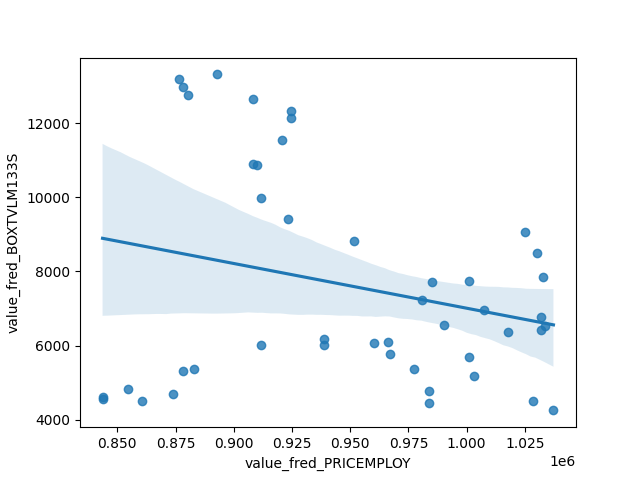
\includegraphics[scale = 0.9]{plots/plot_2026-11-05.png}
\caption{Raw Regression Plot for 2026-11-05}
\end{figure}
\newpage
\subsection{Detrended Regression}
\noindent Regresses the residuals of each series after removing its own linear time trend, so a shared trend can no longer drive the result on its own. A relationship that stays significant here is better evidence of a genuine link between the two series.

\begin{center}
\begin{tabular}{lclc}
\toprule
\textbf{Dep. Variable:}                     & value\_fred\_BOXTVLM133S\_detrended & \textbf{  R-squared:         } &     0.519   \\
\textbf{Model:}                             &                 OLS                 & \textbf{  Adj. R-squared:    } &     0.508   \\
\textbf{Method:}                            &            Least Squares            & \textbf{  F-statistic:       } &     46.42   \\
\textbf{Date:}                              &           Thu, 05 Nov 2026          & \textbf{  Prob (F-statistic):} &  2.40e-08   \\
\textbf{Time:}                              &               19:20:26              & \textbf{  Log-Likelihood:    } &   -369.72   \\
\textbf{No. Observations:}                  &                    45               & \textbf{  AIC:               } &     743.4   \\
\textbf{Df Residuals:}                      &                    43               & \textbf{  BIC:               } &     747.1   \\
\textbf{Df Model:}                          &                     1               & \textbf{                     } &             \\
\textbf{Covariance Type:}                   &              nonrobust              & \textbf{                     } &             \\
\bottomrule
\end{tabular}
\begin{tabular}{lcccccc}
                                            & \textbf{coef} & \textbf{std err} & \textbf{t} & \textbf{P$> |$t$|$} & \textbf{[0.025} & \textbf{0.975]}  \\
\midrule
\textbf{const}                              &   -2.659e-10  &      136.526     & -1.95e-12  &         1.000        &     -275.330    &      275.330     \\
\textbf{value\_fred\_PRICEMPLOY\_detrended} &      -0.0156  &        0.002     &    -6.813  &         0.000        &       -0.020    &       -0.011     \\
\bottomrule
\end{tabular}
\begin{tabular}{lclc}
\textbf{Omnibus:}       &  0.541 & \textbf{  Durbin-Watson:     } &    0.520  \\
\textbf{Prob(Omnibus):} &  0.763 & \textbf{  Jarque-Bera (JB):  } &    0.636  \\
\textbf{Skew:}          & -0.013 & \textbf{  Prob(JB):          } &    0.727  \\
\textbf{Kurtosis:}      &  2.418 & \textbf{  Cond. No.          } & 5.97e+04  \\
\bottomrule
\end{tabular}
%\caption{OLS Regression Results}
\end{center}

Notes: \newline
 [1] Standard Errors assume that the covariance matrix of the errors is correctly specified. \newline
 [2] The condition number is large, 5.97e+04. This might indicate that there are \newline
 strong multicollinearity or other numerical problems.

\begin{figure}
\centering
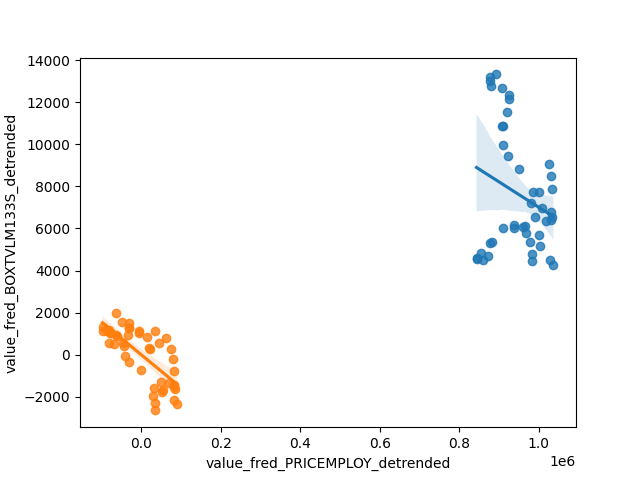
\includegraphics[scale = 0.9]{plots/plot_2026-11-05_detrended.png}
\caption{Detrended Regression Plot for 2026-11-05}
\end{figure}
\newpage
